%%%%%%%%%%%%%%%%%%%%%%%%%%%%%%%%%%%%%%%%%%%%%%%%%%%%%%%%%%%%%%%%
% Sim
%%%%%%%%%%%%%%%%%%%%%%%%%%%%%%%%%%%%%%%%%%%%%%%%%%%%%%%%%%%%%%%%
\section{仿真}
本文使用基于C++的仿真器\cite{olzhn2021}进行仿真。

% ////////////////////////////////////////
\subsection{给定参数计算}
根据给定出发点和到达点的改进春分点轨道根数,
计算可得开普勒轨道根数为
\begin{center}\begin{tabular}{lll}
    \toprule
    名称 & 地球 & 火星 \\
    \midrule
    半长轴    a & $ 1.000840$ & $ 1.523677$ \\
    偏心率    e & $ 0.016507$ & $ 0.093435$ \\
    轨道倾角  i & $ 0.000021$ & $ 0.032276$ \\
    升交点赤经Ω & $ 0.030896$ & $ 0.864609$ \\
    近地点幅角ω & $-1.422358$ & $-1.281742$ \\
    真近点角    & $ 3.824526$ & $ 6.182348$ \\
    $\mu$值     & $398601   $ & $42808    $ \\
    \bottomrule
\end{tabular}\end{center}
可算出以速度为单位的比冲为$I_{sp}=19600$m/s,
也就是说保持发动机推力$F=1$N时,
燃料消耗速度为$d_m=1/19600$千克/秒,
限制发动机工作时间不超过总质量的40\%,
即$T_f=19600*400=7.84\times10^6$秒,约90天。
为统一单位,将长度单位全部换算成km,
则推力为$F=10^{-3}$kN。

% ////////////////////////////////////////
\subsection{建模}
假设探测器在转移轨道上不受地球和火星引力影响。
考虑燃料消耗的火星探测器动力学方程为
\begin{align}
    &\ddot{\vec{r}} = -\frac{\mu_s}{||\vec{r}||^3}\vec{r}
    + \frac{10^{-3}}{m(t)}\epsilon(t)
    \left[\begin{matrix}
        \cos\phi\cos\theta \\ \cos\phi\sin\theta \\ \sin\phi
    \end{matrix}\right] \label{eqSimAcc} \\
    &\dot{m}(t) = -\frac{1}{19600}\epsilon(t) \notag
\end{align}
其中
$\phi$和$\theta$分别为发动机推力向量的俯仰角和方位角,
$\epsilon(t)=0$或$1$表示发动机开机或关机。
建立探测器被控对象模型的模块框图如图\ref{figSimPlant}所示。
\begin{center}
	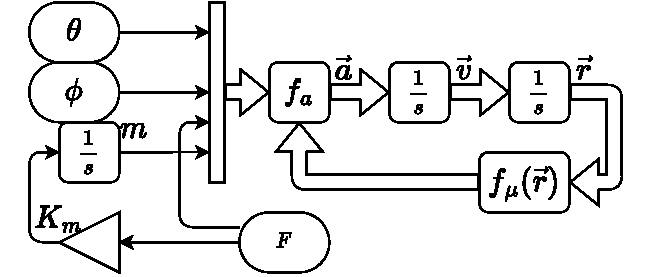
\includegraphics[scale=0.8]{plant.pdf}  \\
	\figcaption{火星探测器被控对象模型的模块框图}\label{figSimPlant}
\end{center}
其中$K_m=-\frac{\bar{d}_m}{\bar{F}}$。
$K_m\cdot F$为燃料消耗速度,作为质量积分器的输入。
有三个输入模块,分别为
发动机方位角$\theta$、俯仰角$\phi$、推力大小$F$,
这三个输入是待优化的时间函数。
函数模块$f_\mu(\vec{r})$计算引力加速度的系数
\[f_\mu(\vec{r})=-\frac{\mu_s}{||\vec{r}||^3}\]
输入为位置向量,输出为标量。
函数模块$f_a$计算加速度向量,即式\eqref{eqSimAcc},
输入为$\theta$、$\phi$、$F$、$m$这4个标量,输出为加速度向量。

% ////////////////////////////////////////
\subsection{仿真调试}
为了验证建模与仿真结果正确,
将部分调试步骤和中间结果记录如下。

\noindent\textbf{绘制轨道}\par
为验证出发点与到达点结果正确,
分别从出发点与到达点开始绘制半个公转周期轨道作为参考,如图\ref{figSimDebug1}所示。
\begin{center}
	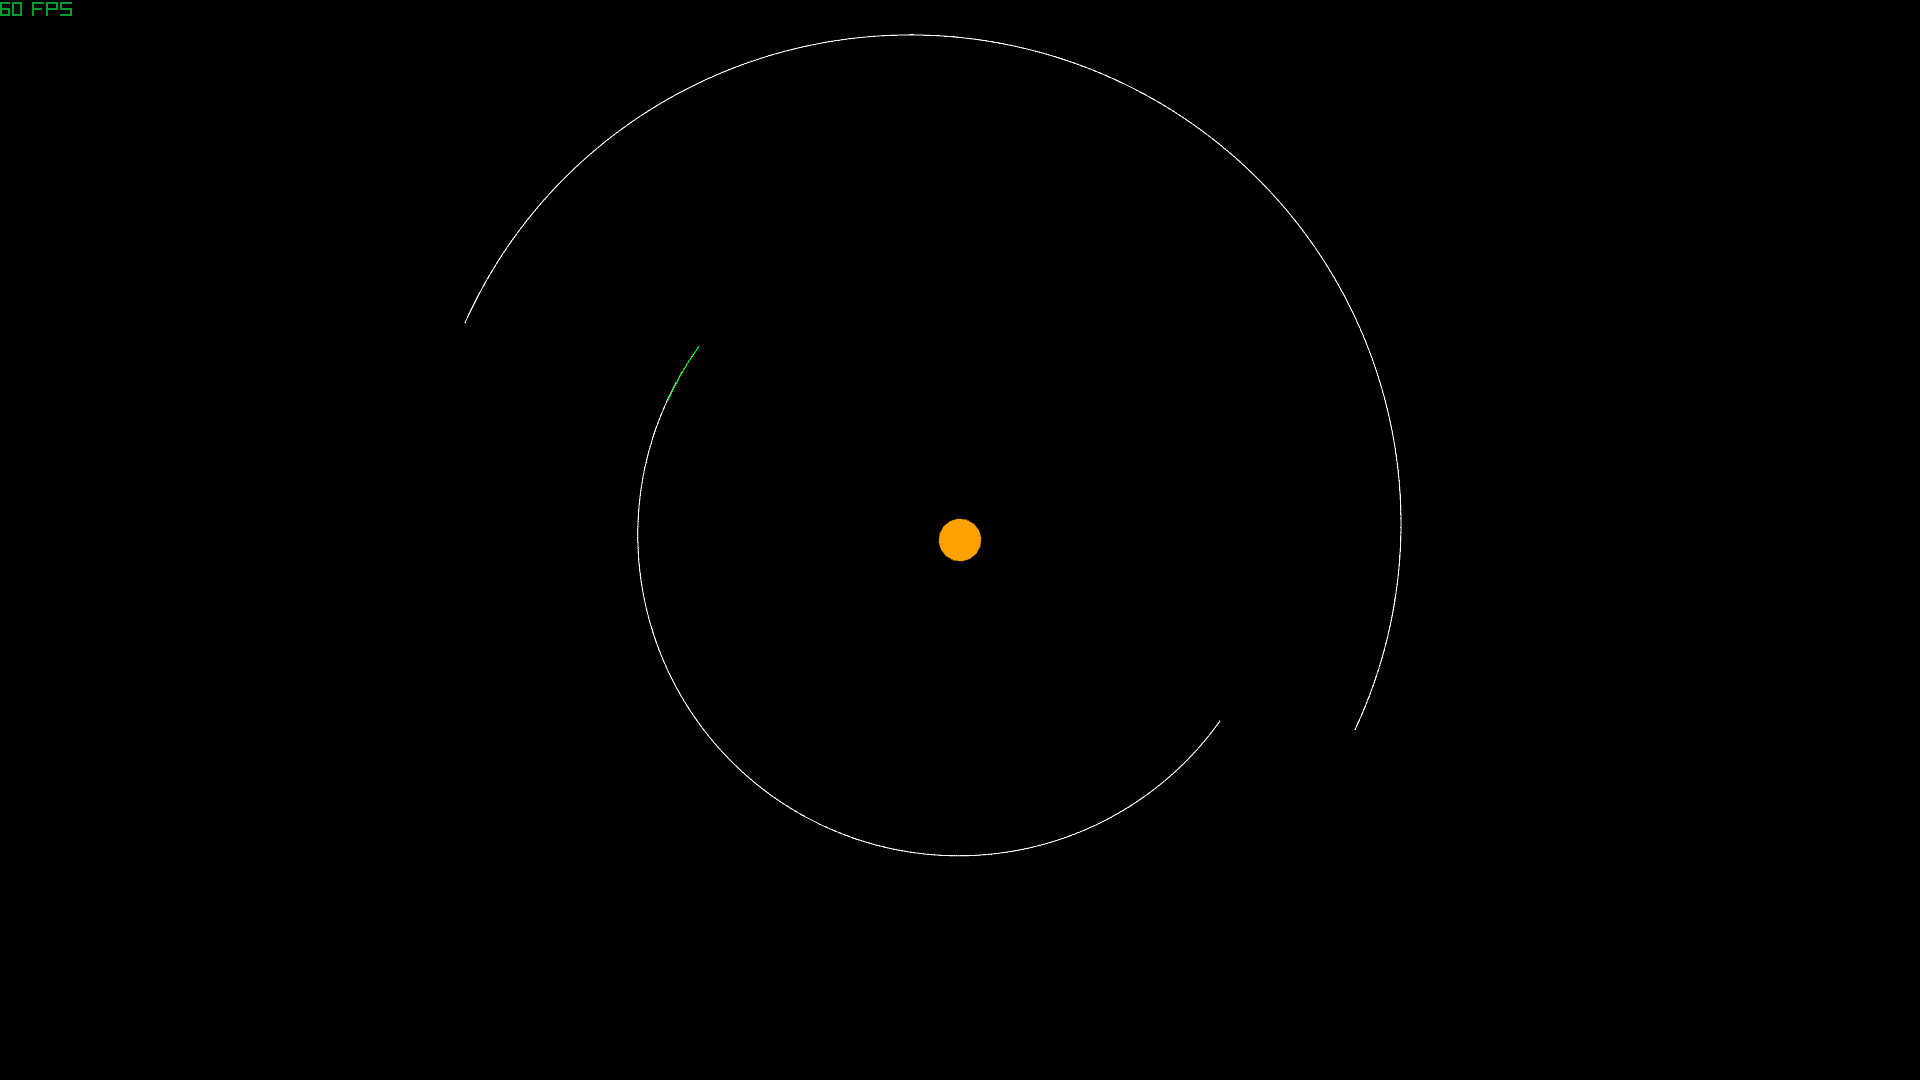
\includegraphics[scale=0.2]{simdebug1.png}  \\
	\figcaption{地球和火星的半个公转周期轨道俯视图}\label{figSimDebug1}
\end{center}
地球和火星的公转周期分别按365天和687天计算,
半个公转周期分别约为$1577$和$2968$仿真器秒。
1仿真器秒等于$1000$仿真步长,
1仿真步长等于实际时间10秒。
仿真器坐标下的出发点位置和速度向量分别为
\[[\begin{matrix}
    -113.102 & 101.033 & 0.00219
\end{matrix}]^\text{T}\]
\[[\begin{matrix}
    -0.19353 & -0.22118 & -4.517067e-06
\end{matrix}]^\text{T}\]
结果基本正确。

\noindent\textbf{燃料消耗}\par
仿真$10^5$个步长后,
仿真得剩余总质量为$948.98$kg。
$10^5$个步长对应$10^6$秒,
计算得燃料消耗$10^6\times\frac{1}{19600}=51.02$kg,
结果正确。
图\ref{figSimDebug1}中的绿色轨迹为
发动机推力俯仰角为0,方位角为$\theta-1.57$时持续工作$10^5$个步长的结果。

% ////////////////////////////////////////
\subsection{结果展示}
使用差分进化算法优化结果如图\ref{figSimAns1}所示。
两图分别为接近俯视图和接近侧视图。
对应的损失函数为$e=352.849$,
从出发点开始的加速段耗时约$6069000$秒,
到达点前的减速段耗时约$1102000$秒,
总质量剩余$634.133$kg。
\begin{center}
	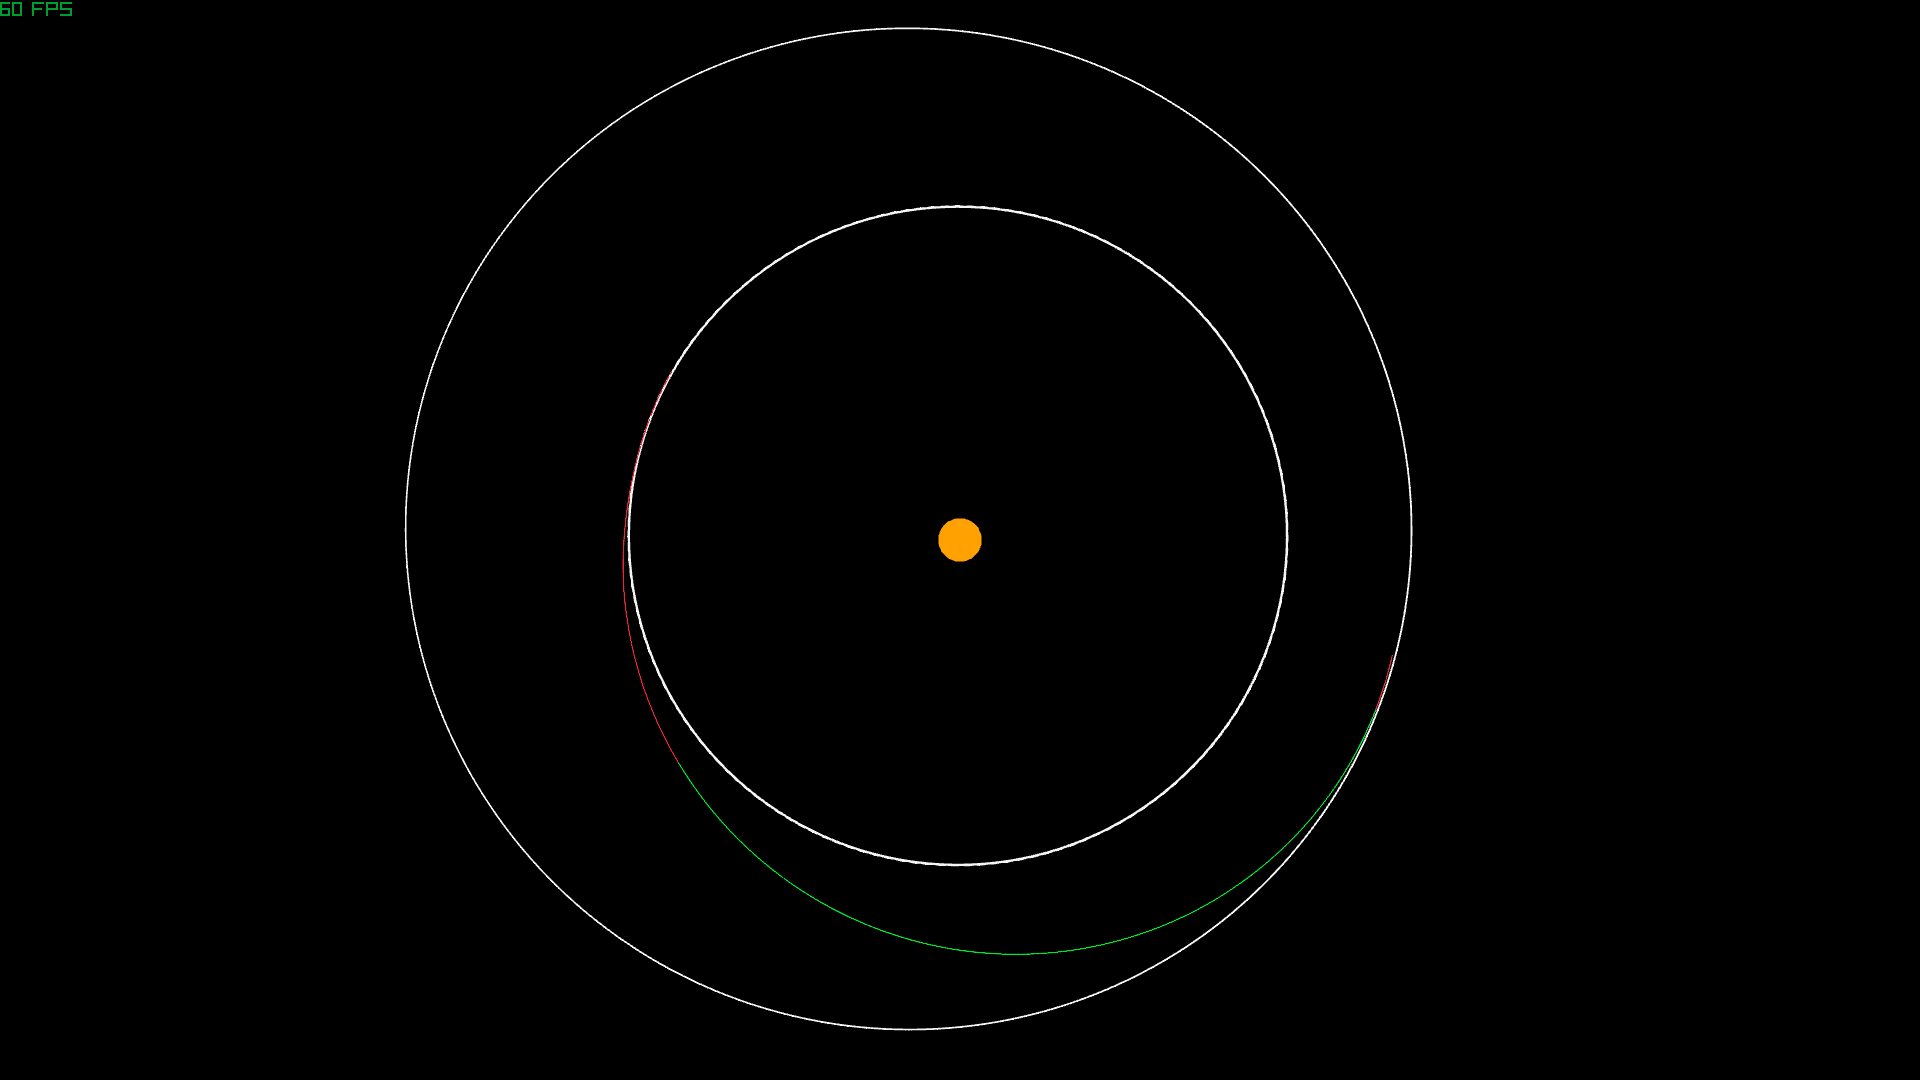
\includegraphics[scale=0.2]{simans1.png}  \\
	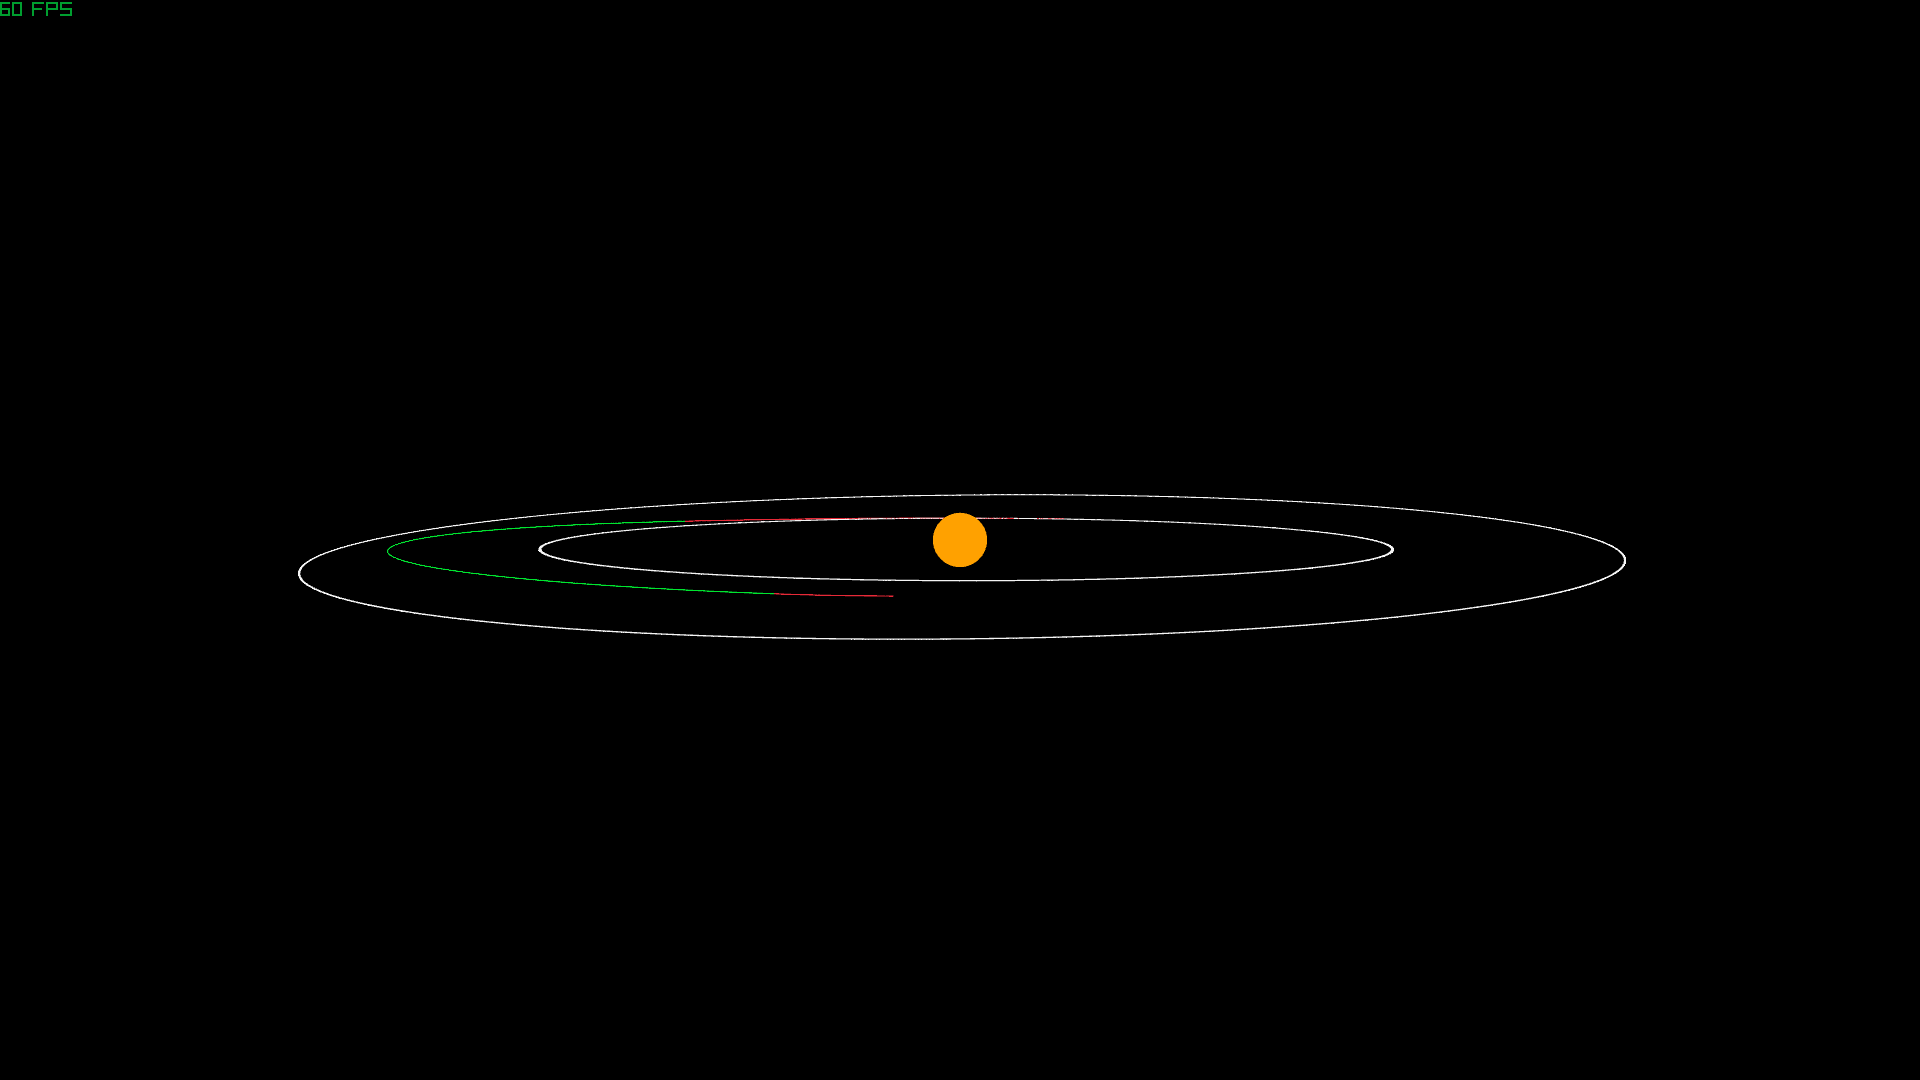
\includegraphics[scale=0.2]{simans2.png}  \\
	\figcaption{差分进化算法优化结果}\label{figSimAns1}
\end{center}
因为优化算法使用的时间单位是$10^6$秒,
是图\ref{figSimDebug1}中的100倍,
所以图\ref{figSimAns1}中地球和火星的轨道画了50圈。

使用模式搜索法优化结果如图\ref{figSimAns2}所示。
此时将损失函数中燃料消耗的比重由$10^{-2}$改为$10^{-3}$,
对应的优化后的损失函数为$e=78.870$,
从出发点开始的加速段耗时约$5778000$秒,
到达点前的减速段耗时约$2458000$秒,
总质量剩余$579.796$kg。
\begin{center}
	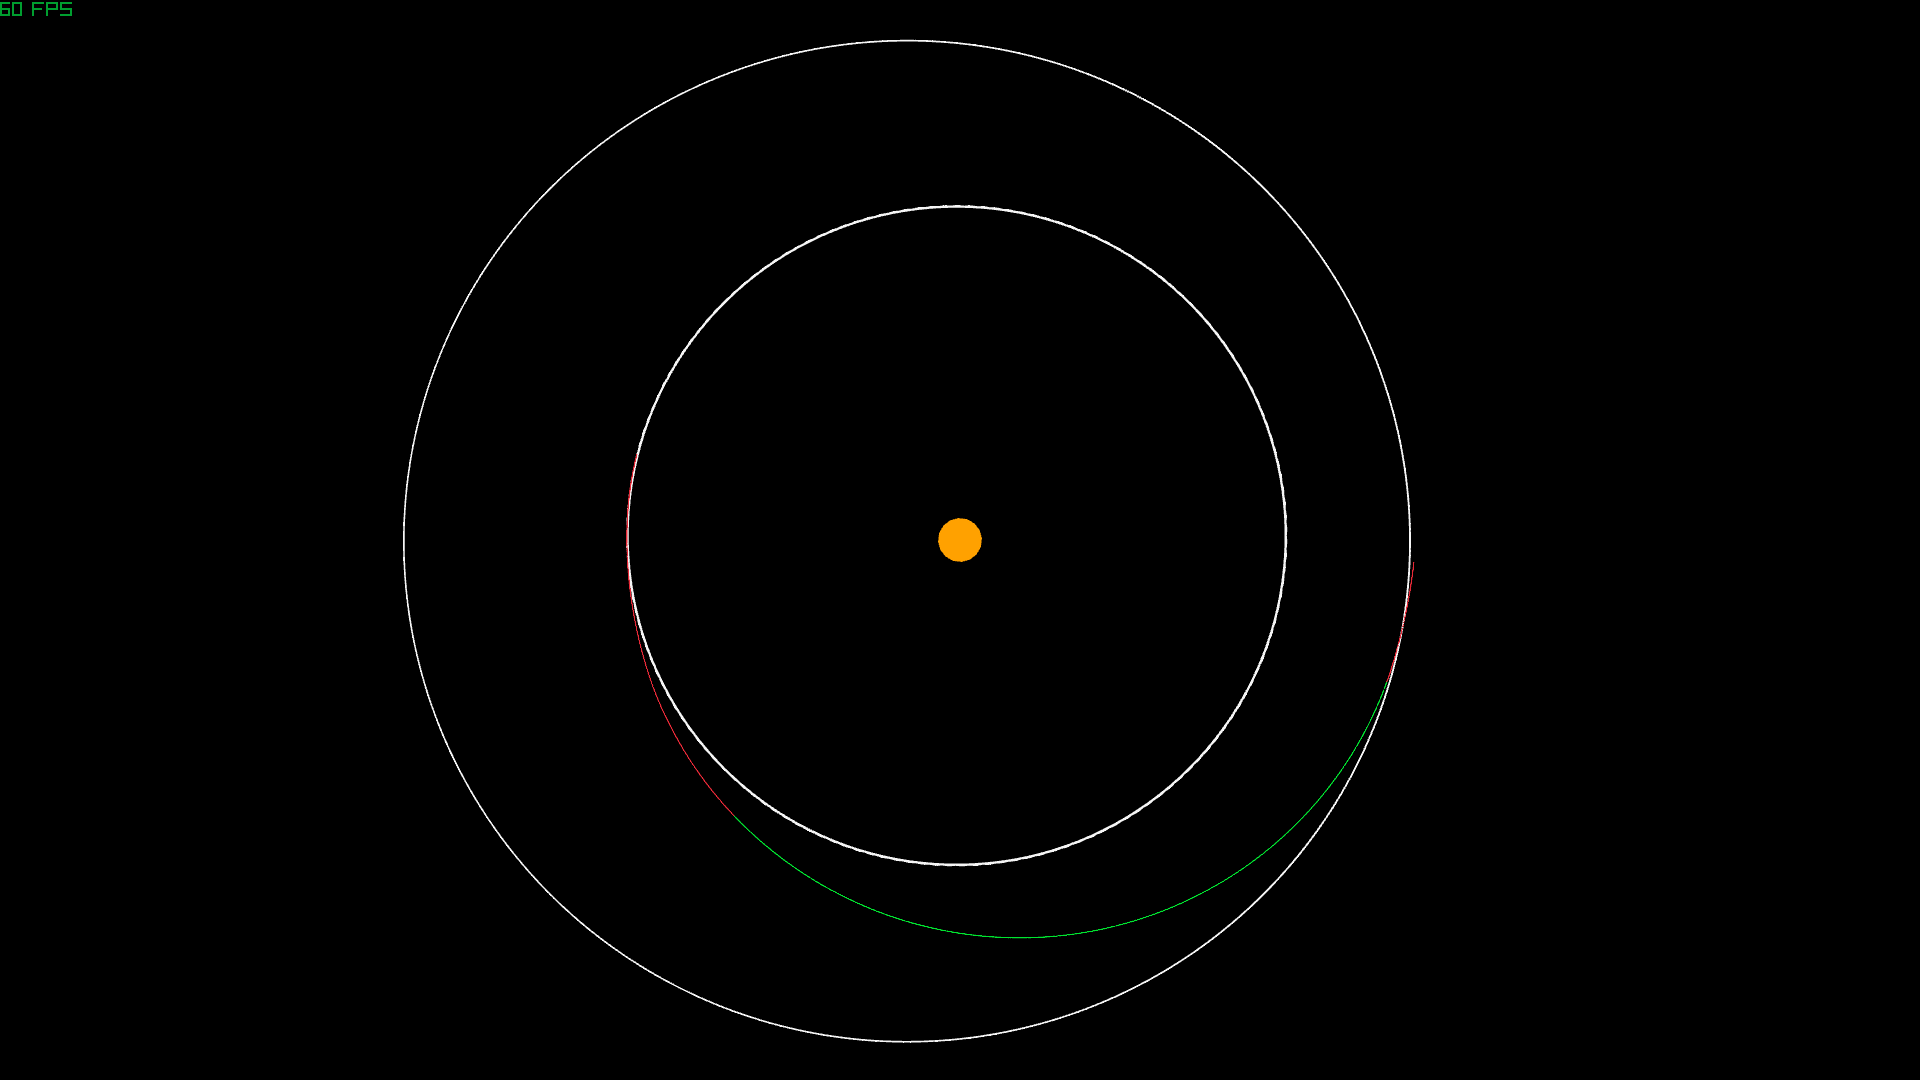
\includegraphics[scale=0.2]{simans3.png}  \\
	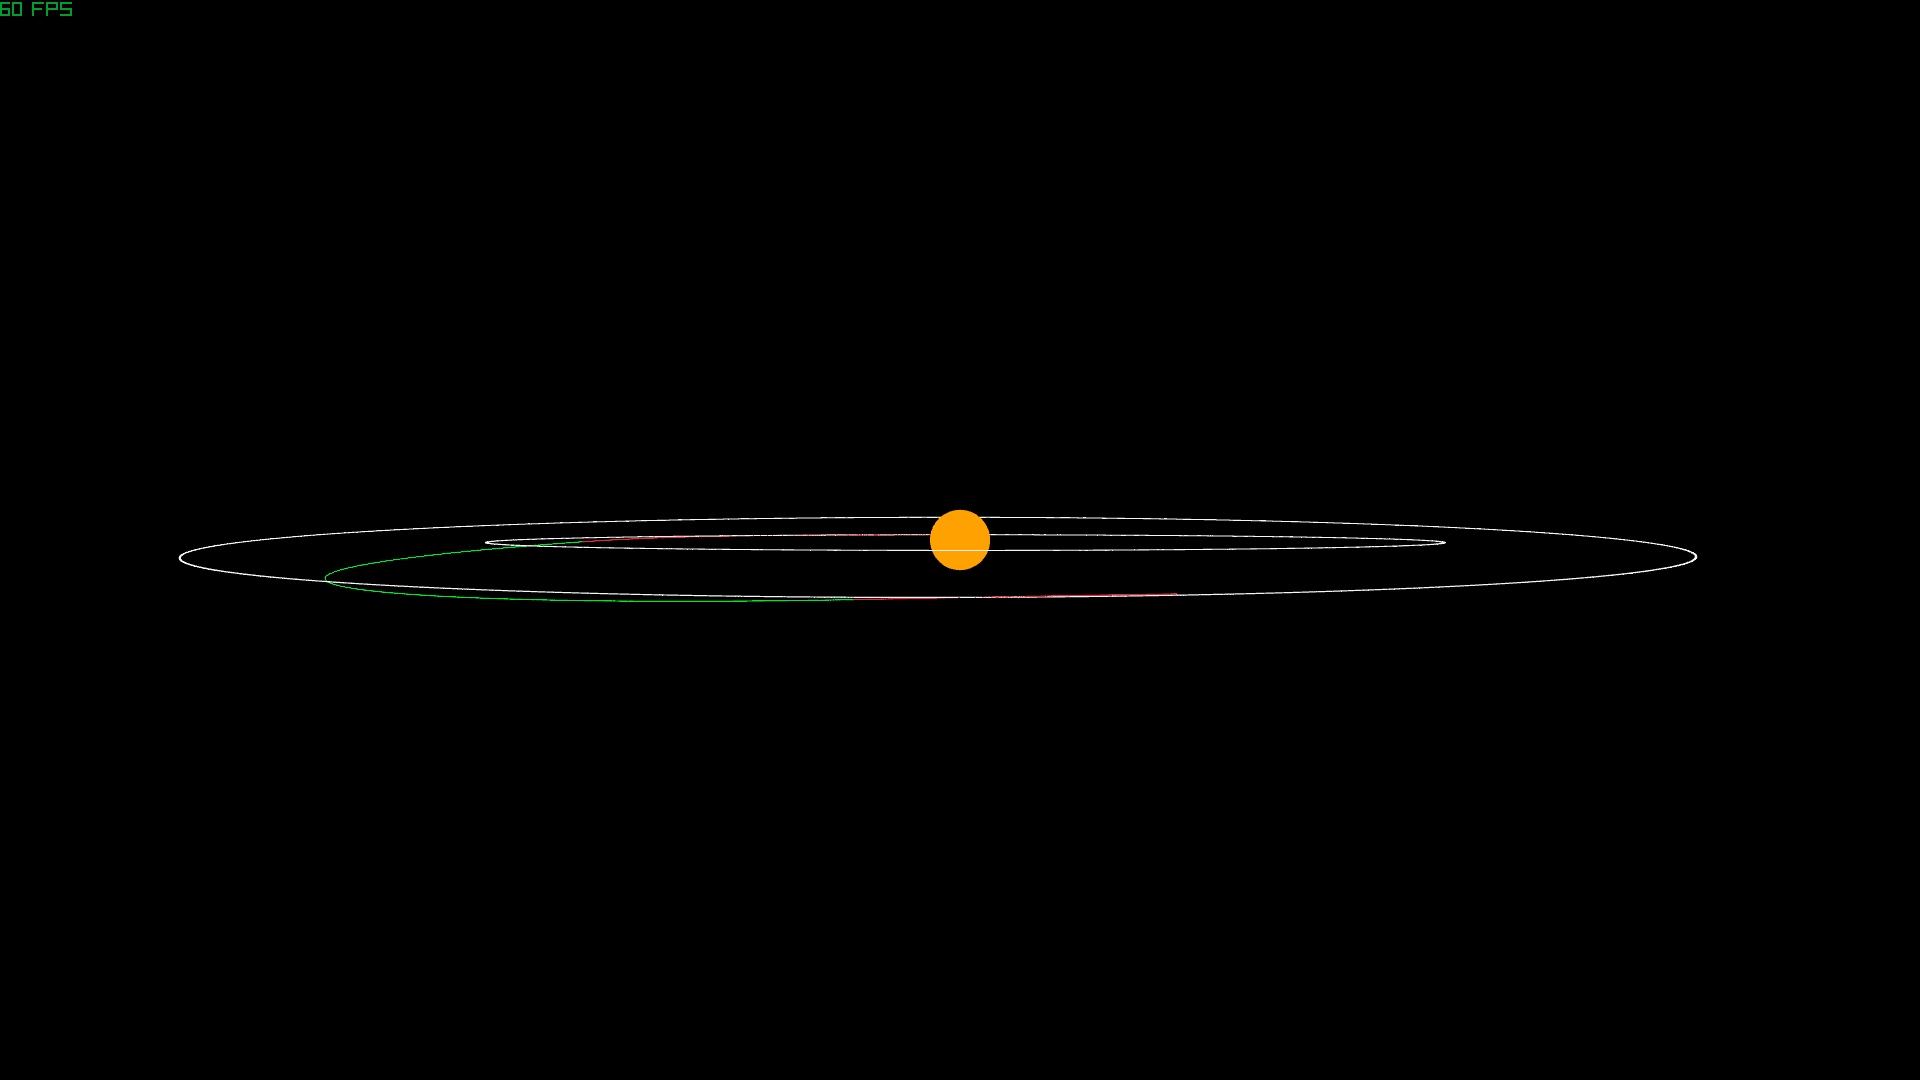
\includegraphics[scale=0.2]{simans4.png}  \\
	\figcaption{模式搜索法优化结果}\label{figSimAns2}
\end{center}

